% vim: ft=tex spell spelllang=en ts=2 sw=2

\cleardoublepage
\setchaptertoc
\chapter{Introduction}

This chapter explains the reasons which motivate the development of this
project, and provides an outline of the goals and planning for its
realization.

\afterintro

\section{Description \& Motivation}

Most programming languages provide some mechanism to use libraries —sometimes
called \emph{modules}— implemented in some other language. Most of the time,
this other language belongs to the family of the C language, which can be
compiled into \emph{native object code}. The reasons are twofold: on one hand
it allows to reuse functionality provided by the system that otherwise would
not be available, and in the other hand it opens the door to implementing
performance--critical pieces of a system using native code.

Despite the advantages, using native code from a different host programming
language requires creating a layer of software often called \emph{bridge}, or
\emph{binding} from now on, which wraps the native library to provide an
interface compatible with the run-time environment of the dynamic programming
language. Those bindings, created either manually or with the help of code
generation tools, need to be compiled before they can be used.

When building native code, compilers are capable of adding
\emph{debugging information} to their output, which can be used to gain
additional insight into a program using a \emph{symbolic debugger}. As
a matter of fact, any other tool capable of understanding the format in which
the compiler writes the debugging information can make use of it for its own
purposes. Among plenty other details about the source program, debugging
information includes descriptions of the functions compiled as part of each
compilation unit, parameters and their corresponding data types, return types,
and the memory layout of the involved user-defined types; which is a superset
of the information needed to invoke those functions. In other words, the
debugging information contains all the details needed to make library bindings
automatically, potentially allowing dynamic programming languages to invoke
native code directly without any kind of human intervention.

% The goal of this project is to implement such an automatic invocation method
% for the Lua programming language, using the debugging information in \Dwarf*
% format as generated by the compiler to allow calling into native code from
% arbitrary libraries at run-time, without needing the presence of previously
% created bindings.


\section{Project Goals}
	\label{sec:project-goals}

The main goal of this project to develop an automatic binding system for the
Lua programming language which allows seamless usage of libraries written in
C at runtime. To achieve this, it will use the debugging information generated
by the C compiler. Additionally:

\begin{itemize}

	\item Modifications to the Lua virtual machine, or its core libraries are to
	be avoided, if possible. The fewer the changes, the lower the maintenance
	cost of the system when Lua is updated. An implementation which does not
	modify Lua itself would be usable with Lua packages provided by the
	operating system, thus easing the setup process.

	\item The implementation will load \gls{ELF} shared objects into the Lua
	virtual machine, and use the debugging information in \gls{DWARF} format
	present in them.

	\item Values of C types, including user defined ones, will be readable and
	modifiable from Lua. It will also be possible to create new values of
	C types from Lua.

	\item Invocation of functions from loaded shared objects will be supported
	for functions of arbitrary return types, and any number of parameters of any
	supported type. Lua values passed to functions will be automatically
	converted to C types whenever possible. Values of C types created from Lua
	will also be accepted as valid function parameters.

	\item The implementation will target the GNU/Linux operating system running
	on the x86\_64 architecture.

	\item The design of the system will be extensible, allowing to add support
	for more shared object formats, debugging information formats, operating
	systems, and architectures.

\end{itemize}


\section{Planning \& Methodologies}
	\label{sec:plan-method}

During the planification phase, the following tasks and subtasks have been
identified:

\begin{enumerate}
	\item Initial study, including:
		\begin{enumerate}
			\item Understanding how different kinds of data are stored in \gls{ELF}
				object files.
			\item Identifying the parts of the \gls{DWARF} specification which apply
				to the scope of the project.
			\item Investigating existing tools which share similar goals.
		\end{enumerate}

	\item Analysis, including:
		\begin{enumerate}
			\item Understanding the relevant parts of the \gls{DWARF}
				debugging information format.
			\item Getting acquainted with Lua and the implementation
				of its \gls{VM}.
		\end{enumerate}

	\item Development, including:
		\begin{enumerate}
			\item Designing the automatic binding system.
			\item Implementing the automatic binding mechanism.
			\item Testing the system, including:
				\begin{itemize}
					\item Designing a set of unit and regressions tests.
					\item Implementing unit and regression tests.
				\end{itemize}
		\end{enumerate}

	\item Validation, including:
		\begin{enumerate}
			\item Developing example Lua programs which demonstrate the
				capabilities of the system.
			\item Rewriting at least one previously existing program to
				validate usage of the system in a real--world scenario.
		\end{enumerate}

	\item Documentation, including writing of the final report.
	% \item Determine whether to use an existing JIT code generator or to
	% 	implement our own.
	% \item Design the JIT code generator.
	% \item Implement the JIT code generator.
\end{enumerate}

For each one of the top-level tasks in the list above,
\autoref{tab:effort-estimate} provides an estimation of the time needed for
the completion, using an effort of eight hours per person, per day (8h/p/d).
For 115 days estimated, the cost of the project would be of 59.000€, using
a price of 65€ per hour.

\begin{table}
	\centering
	\begin{tabular}{rlrr}
		\toprule
		\# & Task & Estimation (days) & Cost (€) \\
		\midrule
		1. & Initial study     & 10 &  5.200 \\
		2. & Analysis          & 15 &  7.800 \\
		3. & Development       & 50 & 26.000 \\
		4. & Validation        & 10 &  5.200 \\
		5. & Documentation     & 30 & 15.600 \\
		\midrule
		   & \emph{Total}      & 115& 59.800 \\
		\bottomrule
	\end{tabular}
	\caption{Effort estimation}
	\label{tab:effort-estimate}
\end{table}

Even though there is only one resource executing the tasks, some techniques
from agile development methodologies are used. Namely:

\begin{itemize}
	\item From Scrum, the concepts of \emph{iteration} and \emph{sprints}, with
    their respective planning and review seasons. Daily stand-up meetings are
    not used, and there is no \emph{scrum master}: none of those would make
    make sense provided that there is only one person in the team.
  \item The \emph{Kanban} methodology is used in order to keep an always
		up to date dashboard with the status of the tasks.
\end{itemize}

\begin{figure}[htH]
	\centering
	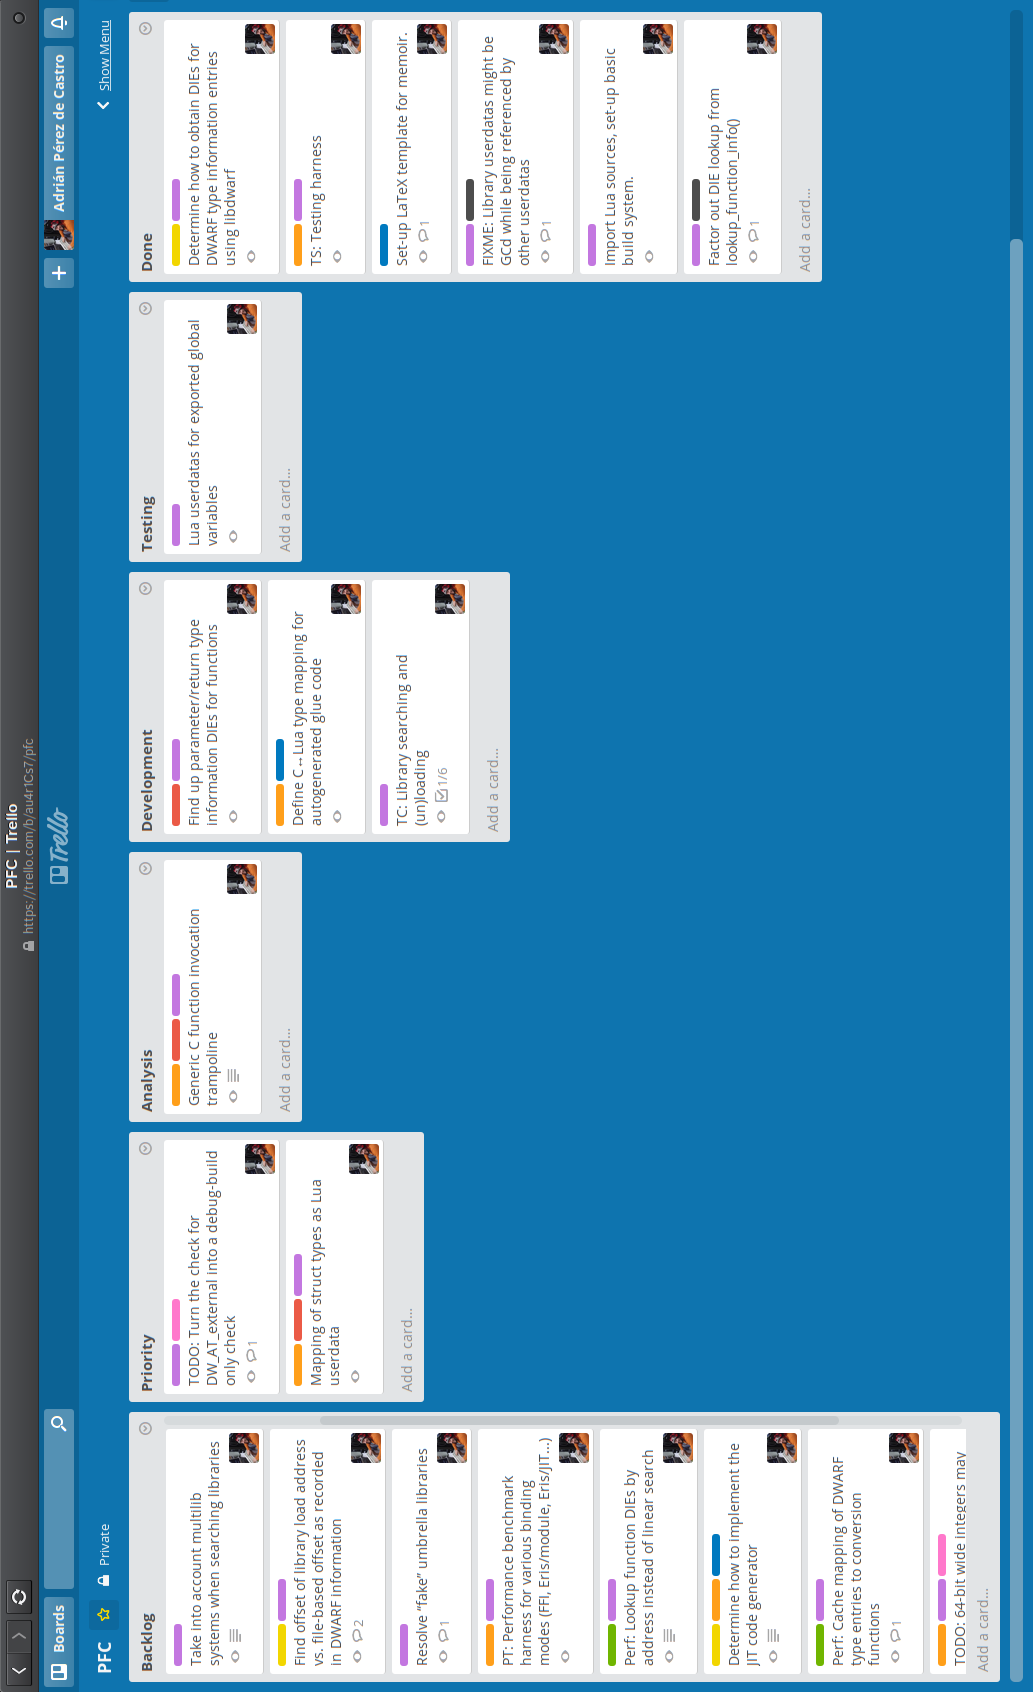
\includegraphics[width=0.8\textwidth]{img/trello-board.png}
	\caption{Kanban board, showing some tasks of this very project}
	\label{fig:kanban-board}
\end{figure}

The Kanban method was invented by \gls{Toyota} to keep the status of
production lines. This methodology keeps a board (physical, in the original
incarnation of the method; nowadays there are even web-based applications like
the one shown in \autoref{fig:kanban-board}) where each element is a task, and
elements are distributed in columns depending on their status. For example,
applied to software development, the columns could be “Pending”, “In
Progress”, “Testing”, and “Finished”. All the tasks are always visible in the
board, so this allows to know the overall status of a project intuitively by
glancing at the board.


\beforeintro
